%% CineRec companion paper — ChinaXiv (ChinaXiv.org) single-column preprint.
%%
%% Rebuilt from the previous acmart/sigconf two-column source to follow the
%% single-column English template of the Chinese Preprint Platform (附件2) and
%% the 2016-02-01 submission-format specification:
%%   * A4, single column; Times New Roman throughout.
%%   * Title 18 pt bold centred, sentence case; authors 12 pt centred with a
%%     "*" marking the corresponding author; affiliations 9 pt, left, with
%%     city + country + postcode.
%%   * Five-part structured abstract (Objective / Methods / Results /
%%     Limitations / Conclusions) at 9 pt, each part its own paragraph.
%%   * Author contribution statement (9 pt) after the affiliations.
%%   * Body sections follow the template order: 1 Introduction, 2 Literature
%%     review, 3 Methodology, 4 Results, 5 Discussion, 6 Conclusion.
%%   * References in the template's author-year-entry style with DOI / URL.
%%   * All figure captions collected on a "Figure Legends" page; each figure
%%     and each table occupies its own page, separated by page breaks, in the
%%     "Figures" and "Tables" sections at the end (spec: 图表编排).
%%   * Figures are white-background 300 dpi renders (docs/paper_*.png), or
%%     white-background line art, so they print correctly.
%%
%% All numeric results are transcribed verbatim from the evaluation artefacts
%% under ``data/``; see ``docs/tech-report.md`` for the single source of truth.
\documentclass[11pt,a4paper]{article}

%% --- page & fonts -----------------------------------------------------------
\usepackage[a4paper,top=25mm,bottom=25mm,left=30mm,right=30mm]{geometry}
\usepackage[T1]{fontenc}
\usepackage[utf8]{inputenc}
\usepackage{txfonts}           % full Times New Roman family (text, maths, tt)
\usepackage{microtype}         % better justification, fewer overfull boxes
\usepackage{graphicx}
\usepackage{booktabs}
\usepackage{array}
\usepackage{amssymb}
\usepackage{xcolor}
\usepackage{tikz}
\usetikzlibrary{arrows.meta,positioning,calc,fit,backgrounds,shapes.geometric}
\usepackage{titlesec}
\usepackage{caption}
\usepackage{enumitem}
\usepackage{url}
\usepackage[hidelinks]{hyperref}

%% Type sizes fixed by the submission spec.
\newcommand{\authfont}{\fontsize{12}{14}\selectfont}
\newcommand{\affilfont}{\fontsize{9}{11}\selectfont}
\newcommand{\absfont}{\fontsize{9}{12}\selectfont}
\newcommand{\contribfont}{\fontsize{9}{12}\selectfont}
\newcommand{\refsfont}{\fontsize{9}{11}\selectfont}
\newcommand{\figfont}{\fontsize{8}{10}\selectfont}
\renewcommand{\footnotesize}{\fontsize{8}{10}\selectfont}  % page footnotes: spec 8 pt

\makeatletter
\renewcommand\normalsize{\@setfontsize\normalsize{10.5}{13.5}}
\makeatother
\normalsize

\setlength{\parindent}{0pt}
\setlength{\parskip}{4pt plus 1pt}
\setlength{\emergencystretch}{2em}

%% Heading sizes (spec): L1 12 pt bold, L2 11 pt bold, L3 10.5 pt bold.
\titleformat{\section}{\normalfont\bfseries\fontsize{12}{14}\selectfont\raggedright}{\thesection.}{0.5em}{}
\titlespacing*{\section}{0pt}{12pt}{5pt}
\titleformat{\subsection}{\normalfont\bfseries\fontsize{11}{13}\selectfont\raggedright}{\thesubsection}{0.5em}{}
\titlespacing*{\subsection}{0pt}{9pt}{4pt}
\titleformat{\subsubsection}{\normalfont\bfseries\fontsize{10.5}{12.5}\selectfont\raggedright}{\thesubsubsection}{0.5em}{}
\titlespacing*{\subsubsection}{0pt}{8pt}{3pt}
\titleformat{name=\section,numberless}{\normalfont\bfseries\fontsize{12}{14}\selectfont\raggedright}{}{0pt}{}

%% First-page footnote without a number (footnote text carries its own "*").
\newcommand\blfootnote[1]{%
  \begingroup
  \renewcommand\thefootnote{}\footnote{#1}%
  \addtocounter{footnote}{-1}%
  \endgroup
}

\captionsetup{font=scriptsize,labelfont=scriptsize,labelsep=period,
              justification=justified,singlelinecheck=false}

\begin{document}

%% --- title block ------------------------------------------------------------
\begin{center}
  {\fontsize{18}{22}\selectfont\bfseries
   CineRec: A practical multi-modal recommender study with cross-dataset
   validation and published-baseline comparison\par}
  \vspace{8pt}
  {\authfont Yulin ZHAO\textsuperscript{1*}\par}
\end{center}
\vspace{4pt}
{\affilfont 1 Independent Researcher, Gongyi 451200, China\par}
\blfootnote{\textsuperscript{*} Corresponding author (E-mail: yulinzhao04@gmail.com).}

%% --- author contribution statement -----------------------------------------
\vspace{6pt}
{\contribfont
\textbf{Author contribution statement.} Yulin ZHAO: proposed the research
question and designed the study, including the model suite, the content-feature
pipeline and the evaluation protocol; implemented the code and carried out all
experiments; collected, cleaned and analysed the data; drafted the manuscript
and revised and approved the final version.\par}

%% --- structured abstract ----------------------------------------------------
\section*{Abstract}
{\absfont
\textbf{Objective:} Many comparative studies in recommender systems are
evaluated on a single dataset and lack statistical validation against published
baselines. This study asks whether model rankings and the contribution of
content features transfer across domains.\par
\textbf{Methods:} We implement six recommenders of increasing complexity
(UserCF, ItemCF, SVD, NeuMF, LightGCN and MultiModalNCF), reproduce two
published baselines (BPR-MF and VBPR) under the same leave-last-5-out protocol,
and evaluate them on MovieLens 100K and an Amazon Video\_Games slice. Neural
models are reported as five-seed mean$\pm$standard deviation, together with
modality-ablation and cold-start studies.\par
\textbf{Results:} The ladder ordering (UserCF $<$ ItemCF $<$ SVD) and the neural
band's lead over SVD hold on both domains; MultiModalNCF is statistically tied
with VBPR. Removing all content costs about one seed standard deviation on
MovieLens and nothing measurable on Amazon, whereas in the cold-start study the
content model clearly outranks the content-blind model.\par
\textbf{Limitations:} Conclusions rest on a single data split without formal
significance testing, epoch budgets are not equalised across models, and the
Amazon slice covers heavy users only.\par
\textbf{Conclusions:} A simple concatenation-based multi-modal extension of
NeuMF is competitive with a published content-aware baseline, and content
features matter mainly for cold-start rather than for overall ranking quality.
The full codebase and evaluation scripts are released for reproduction.\par}

%% --- keywords ---------------------------------------------------------------
\vspace{6pt}
{\fontsize{10.5}{13}\selectfont
\textbf{Keywords:} Recommender systems; Multi-modal recommendation; Cold-start;
Cross-dataset validation; Reproducibility\par}

%% ===========================================================================
\section{Introduction}
Recommender systems are a core component of modern information retrieval,
powering personalised content discovery across e-commerce, media and social
platforms. The field has seen a rapid evolution of methods, from early
collaborative filtering approaches based on user--item interaction matrices to
modern deep learning models that incorporate rich side information such as text
descriptions, images and knowledge graphs.

Despite this rapid progress, many comparative studies in recommender systems
suffer from three limitations: (1) they are evaluated on a single dataset,
limiting the generalisability of conclusions; (2) they lack comparison against
published baselines under matched conditions; and (3) results are often
reported as single-point estimates without statistical significance testing.

In this work we present CineRec, a practical study designed to address these
gaps. Our contributions are as follows:

\begin{enumerate}[leftmargin=2em,itemsep=1pt,topsep=3pt]
  \item We implement and evaluate six recommendation models spanning the full
        evolution from classical neighbourhood methods to deep multi-modal
        models, under a unified evaluation protocol.
  \item We reproduce two published baselines---BPR-MF [1] and VBPR [2]---on the
        same split, allowing direct comparison against established methods.
  \item We validate all conclusions across two datasets, MovieLens 100K and
        Amazon Video\_Games, testing whether observed patterns generalise
        across domains.
  \item We report all neural model results as mean$\pm$standard deviation over
        five random seeds, distinguishing real effects from seed noise.
  \item We conduct both a modality ablation and a cold-start study, quantifying
        the contribution of each content channel.
\end{enumerate}

The study design is summarised in Figure 1. The remainder of this paper is
organised as follows. Section 2 reviews related work. Section 3 describes our
methodology, datasets and evaluation protocol. Section 4 presents the
experimental results. Section 5 discusses the findings and their limitations.
Section 6 concludes.

\section{Literature review}
\subsection{Neighbourhood-based collaborative filtering}
User-based and item-based collaborative filtering [3] are among the earliest and
simplest recommendation approaches. They rely on similarity measures between
users or items to generate recommendations. While simple, they remain
competitive baselines and serve as the foundation for more complex methods.

\subsection{Matrix factorisation}
Matrix factorisation methods such as SVD [4] and BPR [1] transform the
recommendation problem into a latent factor space. BPR, in particular,
introduced a pairwise ranking loss that has become a standard for implicit
feedback recommendation.

\subsection{Neural collaborative filtering}
NeuMF [5] combined matrix factorisation with multi-layer perceptrons to model
non-linear user--item interactions, demonstrating that deep learning can improve
recommendation quality over traditional matrix factorisation.

\subsection{Graph-based recommendation}
LightGCN [6] simplified graph convolutional networks for recommendation by
removing feature transformation and non-linear activation, achieving strong
performance with increased efficiency.

\subsection{Multi-modal recommendation}
VBPR [2] extended BPR with visual features, demonstrating that content
information can improve recommendation accuracy, especially for cold-start
items. Multi-modal recommendation has since become an active research area,
incorporating text, images and other side information.

\section{Methodology (Design/Approach)}
Our objective is to test whether conclusions about model quality and the value
of content features survive two changes that single-dataset studies cannot make:
a second domain, and multi-seed repetition against published baselines. The
methodology below describes the model suite, the shared content features, the
two datasets and the evaluation protocol; all configuration parameters are
listed in Table 1.

\subsection{Datasets}
We conduct experiments on two datasets:

\begin{itemize}[leftmargin=1.6em,itemsep=1pt,topsep=3pt]
  \item \textbf{MovieLens 100K} [7]: 943 users, 1,682 items and 100,000 ratings
        (1--5 scale), restricted to users with $\geq20$ ratings.
  \item \textbf{Amazon Video\_Games} [8]: 2,288 users, 4,753 items and 75,980
        ratings (1--5 scale), restricted to heavy users with $\geq20$ ratings.
\end{itemize}

The Amazon slice is built deterministically from the 5-core Amazon Reviews 2023
Video\_Games dataset by keeping users with $\geq20$ ratings and re-applying the
item 5-core rule. The original 5-core dataset is publicly available from the
Amazon Reviews dataset repository; our slice definition and processing scripts
are included in the codebase.

Poster and overview metadata are retrieved from the TMDB API and remain subject
to TMDB's terms; MovieLens 100K is used under its non-commercial research terms,
and the project's code is released under the MIT licence.

\subsection{Content features}
We precompute content features shared across all content-aware models:

\begin{itemize}[leftmargin=1.6em,itemsep=1pt,topsep=3pt]
  \item \textbf{Text}: Sentence-BERT (all-MiniLM-L6-v2) [9] embeddings of movie
        overviews, 384-dimensional.
  \item \textbf{Image}: ResNet-50 (pool5) [10] embeddings of movie posters,
        2,048-dimensional.
  \item \textbf{Genre}: multi-hot genre vectors, 18-dimensional.
\end{itemize}

\subsection{Model suite}
We evaluate six models of increasing complexity plus two published baselines.
Table 1 summarises all model configurations, and Figure 2 details the
MultiModalNCF architecture. Key details:

\begin{itemize}[leftmargin=1.6em,itemsep=1pt,topsep=3pt]
  \item \textbf{NeuMF}: neural matrix factorisation combining GMF and MLP
        branches.
  \item \textbf{LightGCN}: simplified graph convolutional network with a BPR
        loss.
  \item \textbf{MultiModalNCF}: our multi-modal extension of NeuMF. A content
        tower projects each modality (text 384-d, image 2,048-d, genre 18-d) to
        32 dimensions each, concatenates them to 96 dimensions, then projects to
        32 dimensions before fusing with the behavioural embedding.
  \item \textbf{Positive threshold}: neural models binarise ratings $\geq4$ as
        positive during training.
  \item \textbf{Negative sampling}: four negatives per positive for NeuMF and
        MultiModalNCF; BPR-based models use standard BPR sampling.
\end{itemize}

\subsection{Evaluation protocol}
We use the standard leave-last-5-out split: the five most recent interactions of
each user are held out as the test set. All models are evaluated against the
same candidate set (all items minus the user's training interactions). We report
HR@K and NDCG@K at $K\in\{10,20\}$; Recall@10 is additionally plotted in
Figure 4.

Neural models and both baselines are trained with five random seeds (42--46) and
reported as mean $\pm$ standard deviation. Deterministic models (UserCF, ItemCF,
SVD) have zero spread. Figure 3 summarises the protocol.

\subsection{Implementation, reproducibility and engineering quality}
The pipeline is implemented in Python; content features are precomputed once and
shared by all content-aware models, and every experiment is driven by a
configuration file so that a run is reproducible from its parameters alone.
Experiments run on commodity hardware through the repository's \texttt{make}
targets. To support reproducibility we maintain a well-tested codebase with
continuous integration:

\begin{itemize}[leftmargin=1.6em,itemsep=1pt,topsep=3pt]
  \item \textbf{Test suite}: 125 tests passed with the neural stack installed
        (110 pass and 6 skip without it); line coverage is 50.9\% against a 45\%
        floor. Tests cover data loading, model training loops and evaluation
        metrics.
  \item \textbf{CI pipeline}: three jobs run on every push to main and every
        pull request---linting plus tests with coverage, end-to-end
        accessibility tests, and Docker image builds for both deployment modes
        (lite and full).
  \item \textbf{Dependency hygiene}: we pin version lower bounds to ensure
        reproducible environments. Initial vulnerability scans flagged known
        advisories in transitive dependencies; after updating to patched
        versions, no known vulnerabilities remain (as of October 2026).
  \item \textbf{Documentation}: key architectural decisions are recorded in
        Architecture Decision Records (ADRs), and the codebase provides
        \texttt{make} commands for setup, data preparation, training and
        evaluation, allowing full reproduction from scratch.
  \item \textbf{Repository hygiene}: pre-commit hooks reject large files,
        malformed YAML and merge-conflict markers before each commit, and the
        tracked text files contain no credentials or secret material.
\end{itemize}

\section{Results}
All experimental results below are read from the committed result artefacts of
release v1.0.0 (2026-10-13) and are reproducible via the repository's
\texttt{make} targets; the continuous-integration figures are as reported by the
CI run on v1.0.0.

\subsection{Main results}
Table 2 shows the main model comparison on MovieLens 100K. Key observations:

\begin{itemize}[leftmargin=1.6em,itemsep=1pt,topsep=3pt]
  \item The expected ordering UserCF $<$ ItemCF $<$ SVD holds, with the neural
        band (0.285--0.371 HR@10) sitting above SVD.
  \item BPR-MF and NeuMF are within one combined standard deviation of each
        other.
  \item VBPR's HR@10 edge over MultiModalNCF (0.0055) is smaller than one
        MultiModalNCF standard deviation, while MultiModalNCF leads both NDCG
        columns; the pair is therefore read as statistically tied.
\end{itemize}

Figure 4 visualises the same comparison at $K{=}10$.

\subsection{Modality ablation}
Table 3 shows the modality ablation study on MultiModalNCF. Removing all content
lowers every metric, but by roughly one seed standard deviation. The
single-modality deltas sit inside the noise (one even reverses sign), so no
per-modality ranking is claimed. Figure 5 plots the per-variant HR@10 and
NDCG@10.

\subsection{Cold-start study}
Table 4 shows the cold-start experiment, in which 100 items are removed from
training and evaluated as cold-start items. The ordering content $>$ blind $>$
random holds on every metric. The HR@10 spread of the content variant (0.0290)
exceeds the gap to NeuMF (0.0193), so the margin is reported as a direction
rather than a point magnitude. Figure 6 visualises the three-way comparison.

\subsection{Cross-dataset validation}
Table 5 compares performance across both datasets, and Table 6 repeats the
modality ablation on Amazon.

What transfers: the ladder ordering, the BPR-MF $\approx$ NeuMF tie, the
``single-modality deltas are inside seed noise'' conclusion (on Amazon, removing
any single modality moves HR@10 by at most 0.0030, still inside the 0.0085
full-model spread), and the cold-start direction---the content model reaches
HR@10 0.2364$\pm$0.0202 against 0.1204$\pm$0.0120 for the content-blind model and
0.1092 for random, a content/blind ratio of 1.96$\times$ (1.17$\times$ on
MovieLens). What does not: on Amazon the top HR@10 point estimate belongs to
LightGCN (0.1187 vs 0.1164), a difference well inside the combined spread, and
Behaviour-only $\approx$ Full (0.1163 vs 0.1164).

\subsection{Training cost}
Figure 7 reports the per-model training cost behind Table 2.

\section{Discussion}
\subsection{Key findings}
\begin{enumerate}[leftmargin=2em,itemsep=2pt,topsep=3pt]
  \item \textbf{Model ordering is largely consistent across domains.} The ladder
        backbone (UserCF $<$ ItemCF $<$ SVD) and the neural band's lead over SVD
        hold on both MovieLens and Amazon, suggesting that these patterns are
        not dataset-specific artefacts. Which model leads \emph{within} the
        neural band is domain-dependent, however (VBPR/MultiModalNCF on
        MovieLens, LightGCN on Amazon), so no cross-domain ``best model'' is
        claimed.
  \item \textbf{Content features help in cold-start, but not much in overall
        ranking.} The modality ablation shows that removing content features has
        limited impact on overall ranking quality, whereas the cold-start
        experiments show measurable gains when content is available.
  \item \textbf{MultiModalNCF is competitive with established baselines.}
        Despite using a simple concatenation-based fusion, MultiModalNCF
        performs on par with VBPR, a well-established content-aware baseline.
\end{enumerate}

\subsection{Comparison with published baselines and related work}
Our results are read against two baselines that we reproduce in-house rather
than against their originally reported scores, because the split, the candidate
set and the metric definitions differ across papers. Under this matched
protocol the direction of VBPR's original claim [2] is reproduced: a content-aware
model is clearly stronger than a content-blind model on cold-start items. The
same comparison also bounds that claim---on these two datasets the content
channels contribute little to overall ranking quality, so the advantage of a
multi-modal model over a strong content-blind model such as NeuMF is not
established. This is consistent with the wide-spread observation that visual and
textual side information mainly compensates for missing interaction history.

\subsection{Limitations}
\begin{enumerate}[leftmargin=2em,itemsep=2pt,topsep=3pt]
  \item \textbf{Single split.} We use one leave-last-5-out partition by design;
        conclusions are read against seed spread, not split variance, and no
        cross-validation is performed.
  \item \textbf{No significance testing.} Differences are compared against
        reported standard deviations; formal statistical tests are not run.
        Small deltas (e.g.\ VBPR vs MultiModalNCF HR@10) are explicitly left
        undecided.
  \item \textbf{Epoch budgets are not equalised.} MultiModalNCF runs 10 epochs
        against VBPR's 30 and BPR-MF's/LightGCN's 50, so accuracy comparisons
        carry that asymmetry.
  \item \textbf{Training-time measurement conditions.} Hardware and warm/cold
        cache conditions are not recorded alongside the reported seconds.
  \item \textbf{Second-domain slice represents heavy users only.} The Amazon
        slice is restricted to users with $\geq20$ ratings, chosen to match the
        MovieLens population rule, and does not describe the full Amazon
        population.
  \item \textbf{Content ablation effect is small.} Removing all content costs
        about one seed standard deviation on MovieLens and nothing measurable on
        Amazon.
  \item \textbf{Free-tier deployments sleep when idle.} Reported live behaviour
        may include cold-start latency on the first request.
\end{enumerate}

\section{Conclusion}
We presented CineRec, a practical comparative study of six recommendation models
across two domains, with two published baselines and multi-seed validation. Our
findings confirm that (1) model rankings are largely consistent across datasets,
(2) content features provide measurable benefits in cold-start scenarios but
little overall ranking benefit, and (3) a simple multi-modal extension of NeuMF
can compete with an established content-aware baseline such as VBPR.

Future work includes (1) evaluating on larger-scale datasets such as KuaiRec or
Yelp, (2) exploring more sophisticated fusion strategies beyond simple
concatenation, (3) conducting formal significance testing, and (4) extending the
cold-start study from item cold-start to user cold-start. All code and evaluation
scripts are available at \url{https://github.com/ElijahZhao/cinerec}.

\section*{ACKNOWLEDGEMENTS}
This project was developed as an independent study. The author thanks the
open-source community for providing baseline implementations and datasets.

\textbf{AI use disclosure:} This project was assisted by AI tools throughout
development and manuscript preparation, including code generation, debugging and
documentation writing. The author is solely responsible for the study design,
the verification of all reported results, and the content of this paper.

\section*{References}
\begingroup
\refsfont
\setlength{\parskip}{3pt}
\hangindent=1.7em \hangafter=1

\noindent [1] Rendle, S., Freudenthaler, C., Gantner, Z., \& Schmidt-Thieme, L.
BPR: Bayesian personalized ranking from implicit feedback. In \emph{Proceedings
of the 25th Conference on Uncertainty in Artificial Intelligence (UAI)}.
Arlington, VA: AUAI Press, 2009: 452--461. Retrieved on October 17, 2026, from
\url{https://arxiv.org/abs/1205.2618}.

\noindent [2] He, R., \& McAuley, J. VBPR: Visual Bayesian personalized ranking
from implicit feedback. In \emph{Proceedings of the 30th AAAI Conference on
Artificial Intelligence}. Palo Alto, CA: AAAI Press, 2016: 144--150. DOI:
10.1609/aaai.v30i1.9973.

\noindent [3] Deshpande, M., \& Karypis, G. Item-based top-N recommendation
algorithms. \emph{ACM Transactions on Information Systems}, 2004, 22(1):
143--177. DOI: 10.1145/963770.963776.

\noindent [4] Koren, Y., Bell, R., \& Volinsky, C. Matrix factorization
techniques for recommender systems. \emph{Computer}, 2009, 42(8): 30--37. DOI:
10.1109/MC.2009.263.

\noindent [5] He, X., Liao, L., Zhang, H., Nie, L., Hu, X., \& Chua, T.-S.
Neural collaborative filtering. In \emph{Proceedings of the 26th International
Conference on World Wide Web (WWW)}. Republic and Canton of Geneva:
International World Wide Web Conferences Steering Committee, 2017: 173--182.
DOI: 10.1145/3038912.3052569.

\noindent [6] He, X., Deng, K., Wang, X., Li, Y., Zhang, Y., \& Wang, M.
LightGCN: Simplifying and powering graph convolution network for recommendation.
In \emph{Proceedings of the 43rd International ACM SIGIR Conference on Research
and Development in Information Retrieval}. New York: ACM, 2020: 639--648. DOI:
10.1145/3397271.3401063.

\noindent [7] Harper, F. M., \& Konstan, J. A. The MovieLens datasets: History
and context. \emph{ACM Transactions on Interactive Intelligent Systems}, 2015,
5(4): 19:1--19:19. DOI: 10.1145/2827872.

\noindent [8] Hou, Y., Li, J., He, Z., Yan, A., Chen, X., \& McAuley, J.
Bridging language and items for retrieval and recommendation. \emph{arXiv
preprint}, 2024, arXiv:2403.03952. Retrieved on October 17, 2026, from
\url{https://arxiv.org/abs/2403.03952}.

\noindent [9] Reimers, N., \& Gurevych, I. Sentence-BERT: Sentence embeddings
using Siamese BERT-networks. In \emph{Proceedings of the 2019 Conference on
Empirical Methods in Natural Language Processing (EMNLP-IJCNLP)}. Stroudsburg,
PA: Association for Computational Linguistics, 2019: 3982--3992. DOI:
10.18653/v1/D19-1410.

\noindent [10] He, K., Zhang, X., Ren, S., \& Sun, J. Deep residual learning for
image recognition. In \emph{Proceedings of the 2016 IEEE Conference on Computer
Vision and Pattern Recognition (CVPR)}. Piscataway, NJ: IEEE, 2016: 770--778.
DOI: 10.1109/CVPR.2016.90.

\endgroup

%% ===========================================================================
%% Figure legends (all captions on this page, in order of citation).
%% ===========================================================================
\clearpage
\section*{Figure Legends}
\begingroup
\figfont
\setlength{\parskip}{5pt}
\hangindent=2.2em \hangafter=1

\noindent \textbf{Figure 1.} Overview of the CineRec study. Two domains feed
precomputed text/image/genre content features into a ladder of eight
recommenders---six ladder models plus two reproduced published baselines (marked
$^\star$)---all evaluated under a single leave-last-5-out protocol with five-seed
mean$\pm$std reporting.

\noindent \textbf{Figure 2.} MultiModalNCF architecture (the configuration used
in all reported runs). Behavioural path: GMF over user/item embeddings
($d{=}32$). Content tower: text/image/genre are each projected to 32 dimensions,
concatenated to 96, then projected to a 32-dimensional content embedding; the MLP
path replaces the item embedding with this content embedding. The two paths are
concatenated (64) and mapped to a score. In the cold-start path the GMF item
vector is zeroed, so only the content tower drives scoring.

\noindent \textbf{Figure 3.} Evaluation protocol. A per-user leave-last-5-out
split defines training and held-out interactions; held-out items are ranked
against a candidate set of all non-training items; HR@K and NDCG@K
($K\in\{10,20\}$) are reported over five seeds (42--46) as mean$\pm$std. The
protocol is run independently on both domains.

\noindent \textbf{Figure 4.} Model comparison on MovieLens 100K at $K{=}10$
(HR, NDCG, Recall). The HR@10 and NDCG@10 bars are the five-seed means from
Table 2; Recall@10 is from the same evaluation artefacts.

\noindent \textbf{Figure 5.} Modality ablation on MultiModalNCF (MovieLens 100K):
HR@10 and NDCG@10 for the full model and each ablated variant. The values match
Table 3.

\noindent \textbf{Figure 6.} Cold-start study: 100 items held out of training and
serving as the only candidates, comparing a content-aware model, a content-blind
model and a random ranker. The values match Table 4.

\noindent \textbf{Figure 7.} Training time per model (five-seed means, same runs
as Table 2). Measurement conditions are not recorded; see the limitations in
Section 5.3.

\endgroup

%% ===========================================================================
%% Figures: each figure on its own page, separated by page breaks.
%% ===========================================================================
\clearpage
\section*{Figures}

\clearpage
\begin{center}
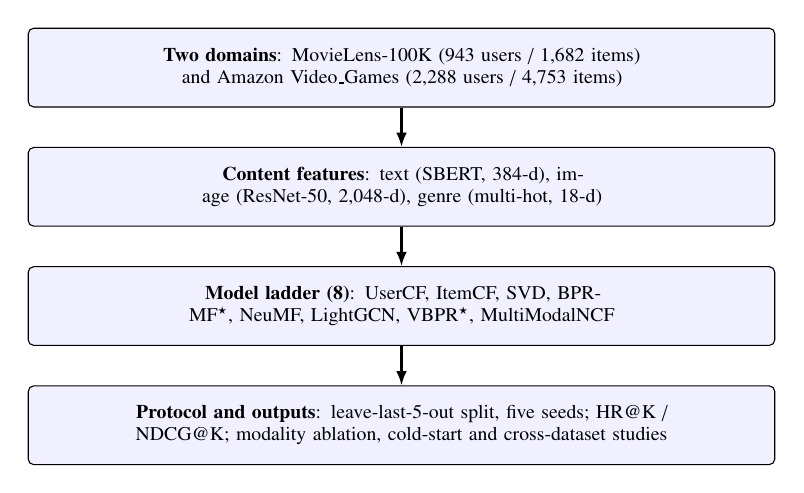
\begin{tikzpicture}[font=\scriptsize,>=Latex,every node/.style={align=center},
    s/.style={draw,rounded corners=2pt,fill=blue!6,inner sep=4pt,
              text width=92mm,minimum height=10mm},
    a/.style={-{Latex[length=1.8mm]},thick}]
  \node[s] (d) {\textbf{Two domains}: MovieLens-100K (943 users / 1,682 items)
    and Amazon Video\_Games (2,288 users / 4,753 items)};
  \node[s,below=5mm of d] (f) {\textbf{Content features}: text (SBERT, 384-d),
    image (ResNet-50, 2,048-d), genre (multi-hot, 18-d)};
  \node[s,below=5mm of f] (m) {\textbf{Model ladder (8)}: UserCF, ItemCF, SVD,
    BPR-MF$^\star$, NeuMF, LightGCN, VBPR$^\star$, MultiModalNCF};
  \node[s,below=5mm of m] (e) {\textbf{Protocol and outputs}:
    leave-last-5-out split, five seeds; HR@K / NDCG@K; modality ablation,
    cold-start and cross-dataset studies};
  \draw[a] (d)--(f);
  \draw[a] (f)--(m);
  \draw[a] (m)--(e);
\end{tikzpicture}
\end{center}

\clearpage
\begin{center}
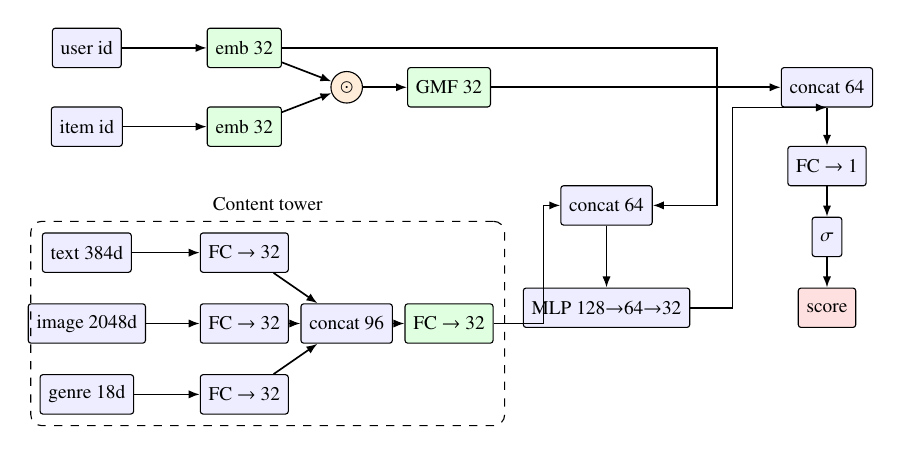
\begin{tikzpicture}[font=\scriptsize,>=Latex,every node/.style={align=center},
    b/.style={draw,rounded corners=1pt,inner sep=3pt,minimum height=5mm,fill=blue!7},
    e/.style={draw,rounded corners=1pt,inner sep=3pt,minimum height=5mm,fill=green!12},
    a/.style={-{Latex[length=1.4mm]},semithick}]
  % behavioural (GMF) path
  \node[b] (uid) at (0,1.0)     {user id};
  \node[e] (eu)  at (2.0,1.0)   {emb 32};
  \node[b] (iid) at (0,0.0)     {item id};
  \node[e] (ei)  at (2.0,0.0)   {emb 32};
  \node[circle,draw,inner sep=1pt,minimum size=4mm,fill=orange!15]
        (dot) at (3.3,0.5) {$\odot$};
  \node[e] (gmf) at (4.6,0.5)   {GMF 32};
  % content tower
  \node[b] (tx) at (0,-1.6) {text 384d};
  \node[b] (im) at (0,-2.5) {image 2048d};
  \node[b] (ge) at (0,-3.4) {genre 18d};
  \node[b] (ftx) at (2.0,-1.6) {FC $\to$ 32};
  \node[b] (fim) at (2.0,-2.5) {FC $\to$ 32};
  \node[b] (fge) at (2.0,-3.4) {FC $\to$ 32};
  \node[b] (cat) at (3.3,-2.5) {concat 96};
  \node[e] (cemb) at (4.6,-2.5) {FC $\to$ 32};
  % MLP path
  \node[b] (mcat) at (6.6,-1.0) {concat 64};
  \node[b] (mlp)  at (6.6,-2.3) {MLP 128$\to$64$\to$32};
  % fusion
  \node[b] (fuse) at (9.4,0.5) {concat 64};
  \node[b] (fc)   at (9.4,-0.5) {FC $\to$ 1};
  \node[b] (sig)  at (9.4,-1.4) {$\sigma$};
  \node[e,fill=red!12] (out) at (9.4,-2.3) {score};
  % edges
  \draw[a] (uid)--(eu);
  \draw[a] (iid)--(ei);
  \draw[a] (eu)--(dot);
  \draw[a] (ei)--(dot);
  \draw[a] (dot)--(gmf);
  \draw[a] (tx)--(ftx); \draw[a] (im)--(fim); \draw[a] (ge)--(fge);
  \draw[a] (ftx)--(cat); \draw[a] (fim)--(cat); \draw[a] (fge)--(cat);
  \draw[a] (cat)--(cemb);
  \draw[a] (eu.east) -- (8.0,1.0) |- (mcat.east);
  \draw[a] (cemb.east) -- (5.8,-2.5) |- (mcat.west);
  \draw[a] (mcat)--(mlp);
  \draw[a] (gmf.east) -- (fuse.west);
  \draw[a] (mlp.east) -- (8.2,-2.3) |- (fuse.south);
  \draw[a] (fuse)--(fc); \draw[a] (fc)--(sig); \draw[a] (sig)--(out);
  \node[draw,dashed,rounded corners,fit=(tx)(ftx)(fge)(cat)(cemb),inner sep=4pt,
        label={[font=\scriptsize]above:Content tower}] {};
\end{tikzpicture}
\end{center}

\clearpage
\begin{center}
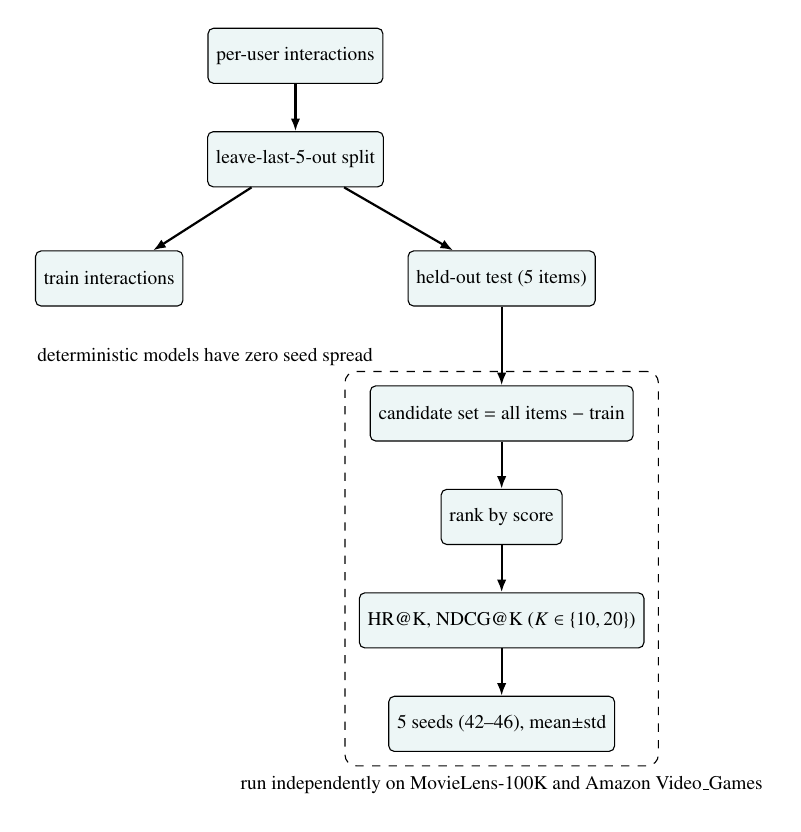
\begin{tikzpicture}[font=\scriptsize,>=Latex,every node/.style={align=center},
    b/.style={draw,rounded corners=2pt,fill=teal!7,inner sep=3pt,minimum height=7mm},
    a/.style={-{Latex[length=1.6mm]},thick}]
  \node[b] (rat) {per-user interactions};
  \node[b,below=6mm of rat] (split) {leave-last-5-out split};
  \node[b,below left=8mm and 3mm of split] (train) {train interactions};
  \node[b,below right=8mm and 3mm of split] (test) {held-out test (5 items)};
  \node[b,below=10mm of test] (cand) {candidate set $=$ all items $-$ train};
  \node[b,below=6mm of cand] (rank) {rank by score};
  \node[b,below=6mm of rank] (met) {HR@K, NDCG@K ($K\in\{10,20\}$)};
  \node[b,below=6mm of met] (seed) {5 seeds (42--46), mean$\pm$std};
  \draw[a] (rat)--(split);
  \draw[a] (split)--(train);
  \draw[a] (split)--(test);
  \draw[a] (test)--(cand);
  \draw[a] (cand)--(rank);
  \draw[a] (rank)--(met);
  \draw[a] (met)--(seed);
  \node[draw,dashed,rounded corners,fit=(cand)(rank)(met)(seed),inner sep=5pt,
        label={[font=\scriptsize]below:run independently on MovieLens-100K and
        Amazon Video\_Games}] {};
  \node[font=\scriptsize,anchor=north west] at ($(train.south west)+(-1mm,-4mm)$)
        {deterministic models have zero seed spread};
\end{tikzpicture}
\end{center}

\clearpage
\begin{center}
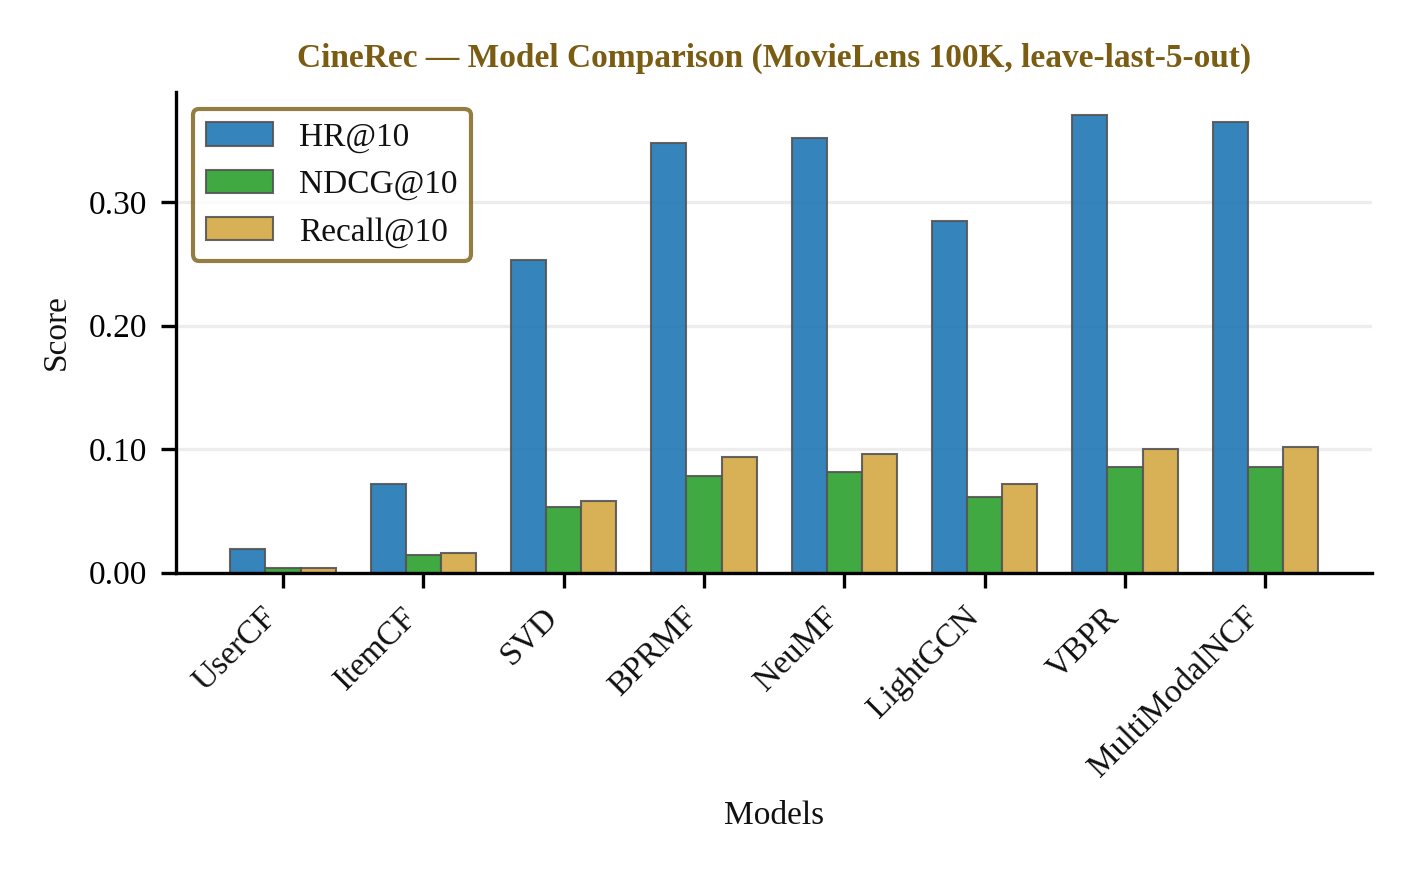
\includegraphics[width=120mm]{paper_model_comparison.png}
\end{center}

\clearpage
\begin{center}
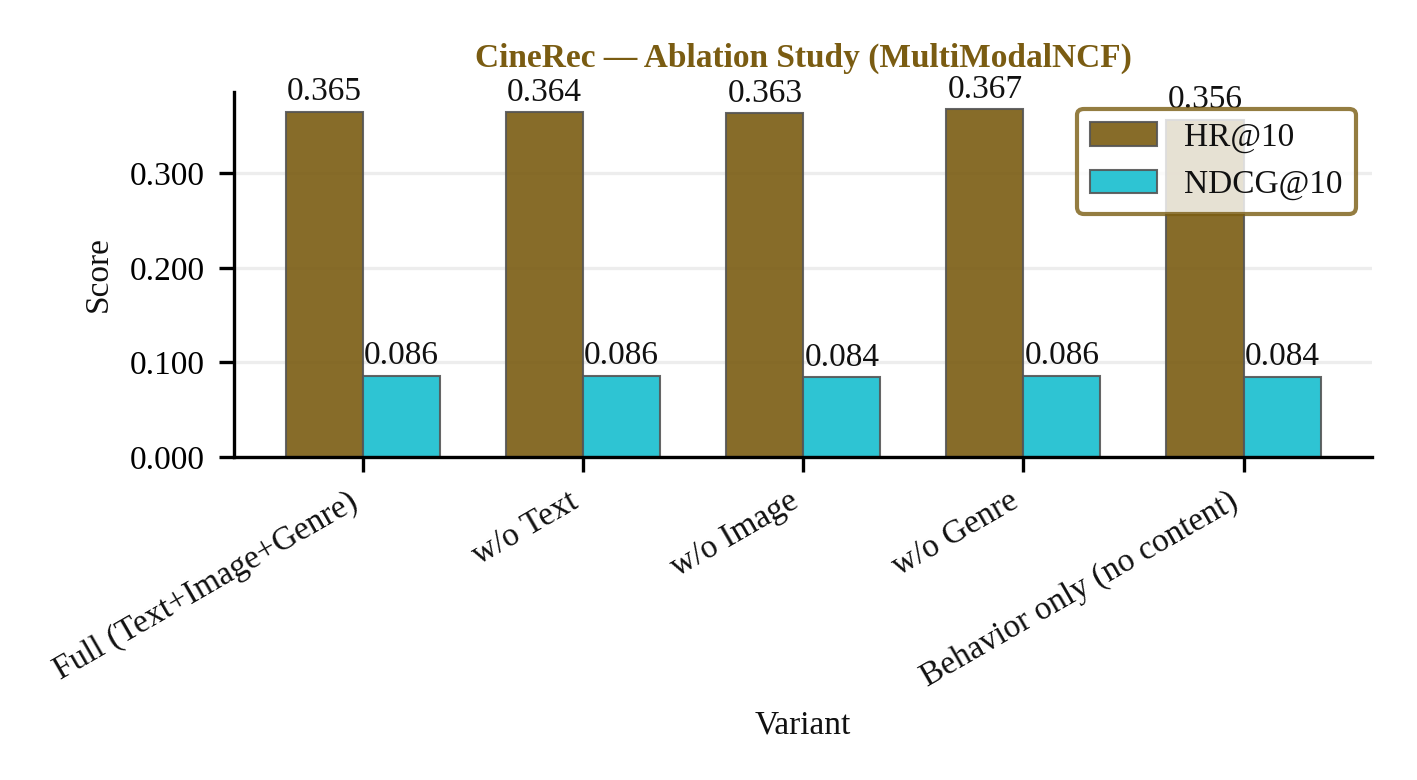
\includegraphics[width=120mm]{paper_ablation_study.png}
\end{center}

\clearpage
\begin{center}
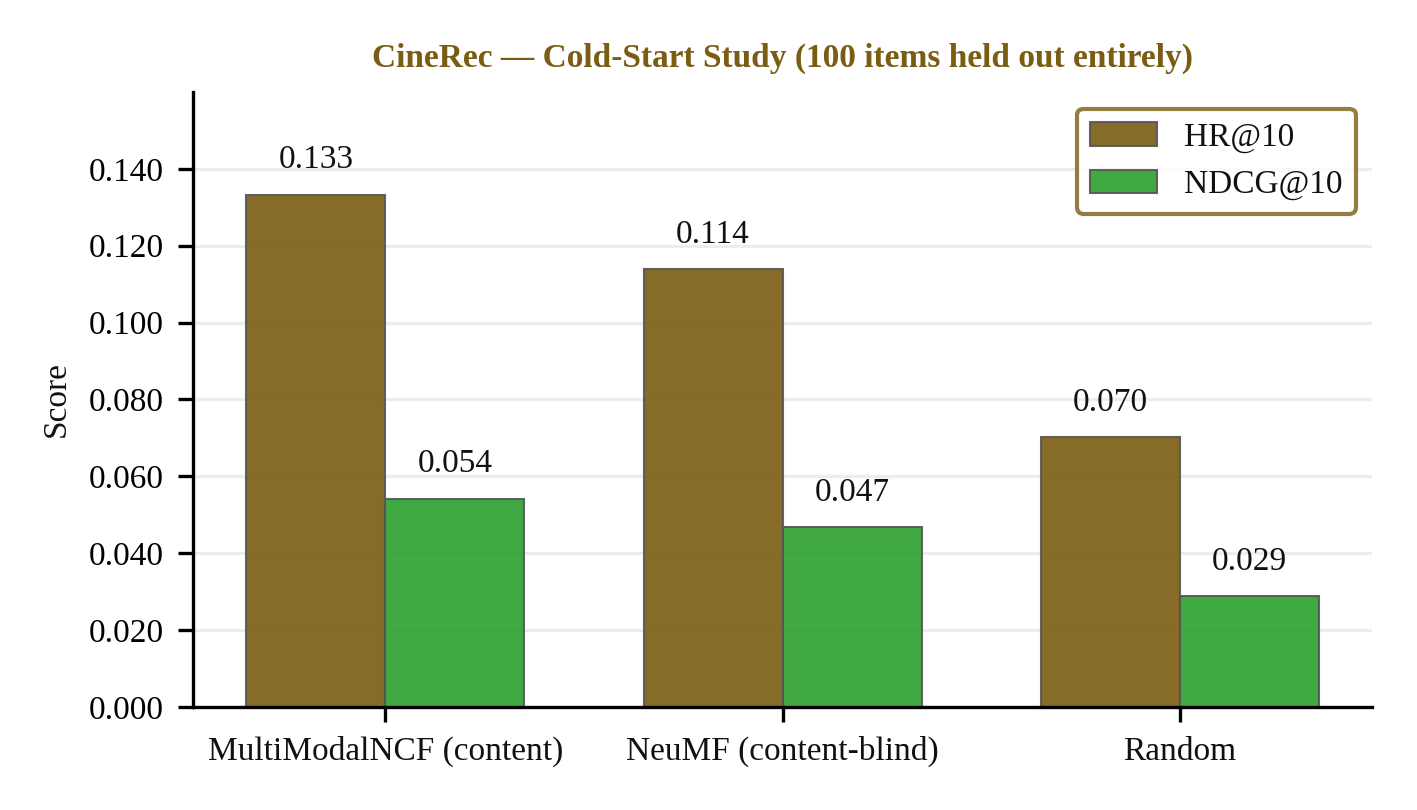
\includegraphics[width=120mm]{paper_coldstart.png}
\end{center}

\clearpage
\begin{center}
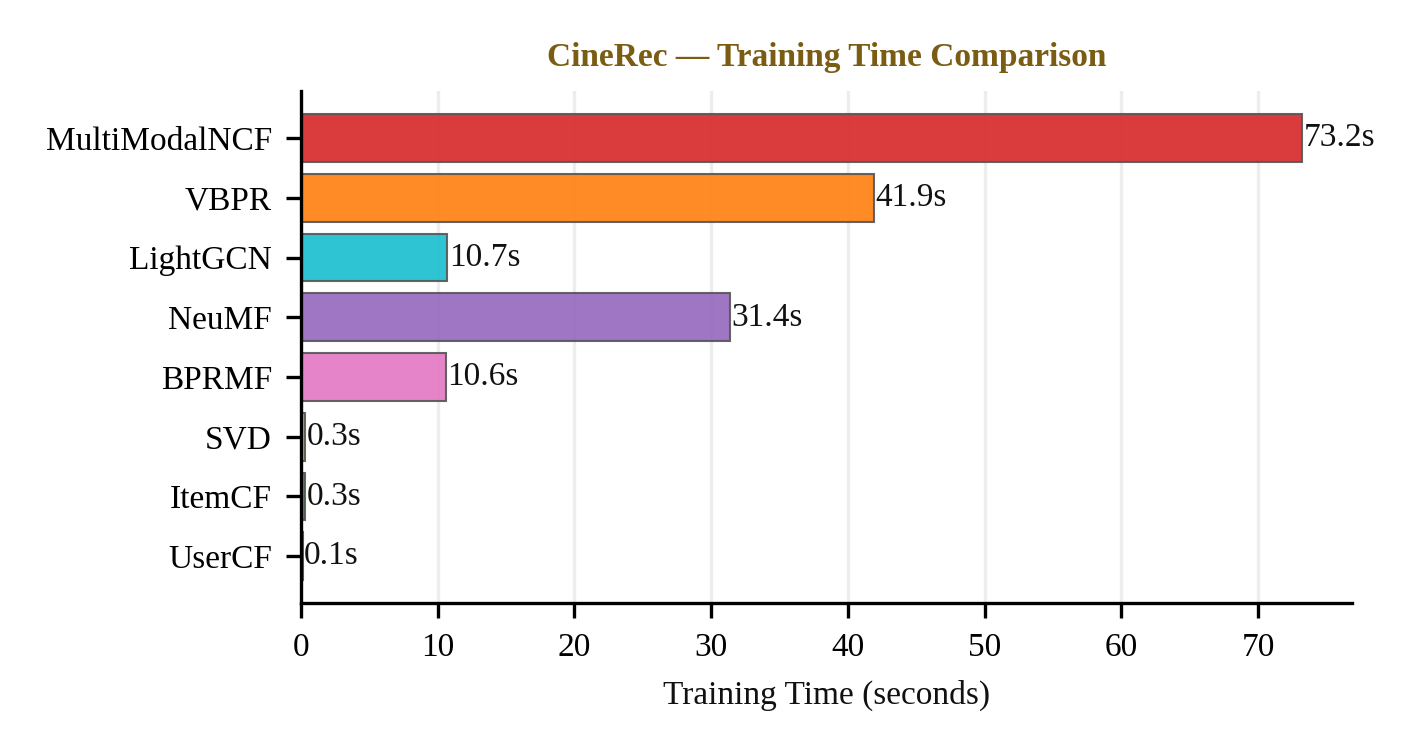
\includegraphics[width=120mm]{paper_training_time.png}
\end{center}

%% ===========================================================================
%% Tables: each table on its own page, separated by page breaks.
%% ===========================================================================
\clearpage
\section*{Tables}

\clearpage
\noindent{\figfont\textbf{Table 1.} Model configurations.}\par
\vspace{4pt}
\begin{center}
{\figfont
\begin{tabular}{@{}p{32mm}p{98mm}@{}}
  \toprule
  Model & Configuration \\
  \midrule
  UserCF & Pearson similarity, $k=50$ neighbours \\
  ItemCF & Adjusted cosine similarity, $k=50$ neighbours \\
  SVD & Truncated SVD, $k=64$ latent dimensions \\
  BPR-MF & dim 64, epochs 50, lr 0.001, batch 4,096, patience 8 \\
  NeuMF & dim 32, MLP (128, 64, 32), epochs 10, batch 512, four negatives,
          patience 3 \\
  LightGCN & dim 64, three layers, epochs 50, batch 4,096, BPR objective,
          patience 8 \\
  VBPR & behaviour dim 64, visual dim 64, epochs 30, lr 0.005 \\
  MultiModalNCF & dim 32, MLP (128, 64, 32), epochs 10, batch 512; content
          tower projects 384/2,048/18 $\to$ 32 each, concatenated (96) $\to$ 32 \\
  \bottomrule
\end{tabular}}
\end{center}

\clearpage
\noindent{\figfont\textbf{Table 2.} Model comparison on MovieLens 100K
(mean$\pm$std over five seeds; training time in seconds).}\par
\vspace{4pt}
\begin{center}
{\figfont
\begin{tabular}{@{}lrrrrr@{}}
  \toprule
  Model & HR@10 & NDCG@10 & HR@20 & NDCG@20 & Train time (s) \\
  \midrule
  UserCF       & 0.0191$\pm$0.0000 & 0.0035$\pm$0.0000 & 0.0477$\pm$0.0000 & 0.0060$\pm$0.0000 & 0.1 \\
  ItemCF       & 0.0721$\pm$0.0000 & 0.0142$\pm$0.0000 & 0.1283$\pm$0.0000 & 0.0199$\pm$0.0000 & 0.3 \\
  SVD          & 0.2534$\pm$0.0000 & 0.0532$\pm$0.0000 & 0.3542$\pm$0.0000 & 0.0664$\pm$0.0000 & 0.3 \\
  BPR-MF       & 0.3476$\pm$0.0116 & 0.0785$\pm$0.0018 & 0.4831$\pm$0.0116 & 0.1034$\pm$0.0018 & 10.6 \\
  NeuMF        & 0.3516$\pm$0.0036 & 0.0814$\pm$0.0016 & 0.4978$\pm$0.0073 & 0.1083$\pm$0.0017 & 31.4 \\
  LightGCN     & 0.2850$\pm$0.0041 & 0.0614$\pm$0.0004 & 0.4250$\pm$0.0047 & 0.0816$\pm$0.0007 & 10.7 \\
  VBPR         & 0.3705$\pm$0.0048 & 0.0855$\pm$0.0009 & 0.5200$\pm$0.0096 & 0.1130$\pm$0.0008 & 41.9 \\
  MultiModalNCF & 0.3650$\pm$0.0077 & 0.0859$\pm$0.0017 & 0.5073$\pm$0.0148 & 0.1144$\pm$0.0015 & 73.2 \\
  \bottomrule
\end{tabular}}
\end{center}

\clearpage
\noindent{\figfont\textbf{Table 3.} Modality ablation on MultiModalNCF
(MovieLens 100K).}\par
\vspace{4pt}
\begin{center}
{\figfont
\begin{tabular}{@{}lrrrr@{}}
  \toprule
  Variant & HR@10 & NDCG@10 & HR@20 & NDCG@20 \\
  \midrule
  Full           & 0.3650$\pm$0.0077 & 0.0859$\pm$0.0017 & 0.5073$\pm$0.0148 & 0.1144$\pm$0.0015 \\
  w/o Text       & 0.3642$\pm$0.0100 & 0.0855$\pm$0.0024 & 0.5075$\pm$0.0108 & 0.1144$\pm$0.0025 \\
  w/o Image      & 0.3631$\pm$0.0085 & 0.0842$\pm$0.0026 & 0.5080$\pm$0.0029 & 0.1132$\pm$0.0025 \\
  w/o Genre      & 0.3673$\pm$0.0080 & 0.0857$\pm$0.0015 & 0.5107$\pm$0.0139 & 0.1144$\pm$0.0016 \\
  Behaviour only & 0.3565$\pm$0.0061 & 0.0844$\pm$0.0024 & 0.4931$\pm$0.0089 & 0.1123$\pm$0.0033 \\
  \bottomrule
\end{tabular}}
\end{center}

\clearpage
\noindent{\figfont\textbf{Table 4.} Cold-start performance (100 items removed
from training).}\par
\vspace{4pt}
\begin{center}
{\figfont
\begin{tabular}{@{}lrrrr@{}}
  \toprule
  Model & HR@10 & NDCG@10 & HR@20 & NDCG@20 \\
  \midrule
  MultiModalNCF (content) & 0.1333$\pm$0.0290 & 0.0542$\pm$0.0151 & 0.2754$\pm$0.0233 & 0.0882$\pm$0.0139 \\
  NeuMF (content-blind)   & 0.1140$\pm$0.0147 & 0.0467$\pm$0.0069 & 0.2351$\pm$0.0129 & 0.0739$\pm$0.0038 \\
  Random                  & 0.0702            & 0.0288            & 0.2018            & 0.0610 \\
  \bottomrule
\end{tabular}}
\end{center}

\clearpage
\noindent{\figfont\textbf{Table 5.} Cross-dataset validation: HR@10 / NDCG@10
comparison.}\par
\vspace{4pt}
\begin{center}
{\figfont
\begin{tabular}{@{}lrrrr@{}}
  \toprule
  Model & ML-100K HR@10 & Amazon HR@10 & ML-100K NDCG@10 & Amazon NDCG@10 \\
  \midrule
  UserCF        & 0.0191 & 0.0122 & 0.0035 & 0.0017 \\
  ItemCF        & 0.0721 & 0.0214 & 0.0142 & 0.0035 \\
  SVD           & 0.2534 & 0.0651 & 0.0532 & 0.0116 \\
  BPR-MF        & 0.3476 & 0.1055 & 0.0785 & 0.0198 \\
  NeuMF         & 0.3516 & 0.1053 & 0.0814 & 0.0190 \\
  LightGCN      & 0.2850 & 0.1187 & 0.0614 & 0.0222 \\
  VBPR          & 0.3705 & 0.1097 & 0.0855 & 0.0196 \\
  MultiModalNCF & 0.3650 & 0.1164 & 0.0859 & 0.0213 \\
  \bottomrule
\end{tabular}}
\end{center}

\clearpage
\noindent{\figfont\textbf{Table 6.} Modality ablation on Amazon Video\_Games
(MultiModalNCF, HR@10, mean$\pm$std over five seeds).}\par
\vspace{4pt}
\begin{center}
{\figfont
\begin{tabular}{@{}lr@{}}
  \toprule
  Variant & HR@10 \\
  \midrule
  Full           & 0.1164$\pm$0.0085 \\
  w/o Text       & 0.1159$\pm$0.0050 \\
  w/o Image      & 0.1177$\pm$0.0033 \\
  w/o Genre      & 0.1194$\pm$0.0017 \\
  Behaviour only & 0.1163$\pm$0.0011 \\
  \bottomrule
\end{tabular}}
\end{center}

\end{document}
